\chapter{Welcome!}
\label{chap:welcome}
Hello folks, and welcome to the exciting world of electric circuits! In this course, you will learn 90\% of everything you would need to be a pro in this exciting field.\footnote{I made this statistic up, but I think it's true.} And if you are doubting me in my description of this course and its subject matter as ``exciting'', let me borrow the words of Jesus Himself and say, ``stop doubting and believe\footnote{John 20:27}''. Yes, I \textit{did} just go there. 
\par
First things first---you will likely get overwhelmed in this course by all of the material we cover. However, I promise you, it's all connected, and I think it helps to think about just \textit{how} everything in electric circuits and electronics is connected before we dive in.
\par
\textbf{When you feel confused, remember that all circuits you will encounter in life fit into just two categories:}
\begin{itemize} 
\item \textbf{circuits that deliver power to something}
\item \textbf{circuits that condition signals (i.e., manipulate information)}
\end{itemize}

Some circuits fit neatly into one or the other of these categories while some circuits fit into both, but no circuits fit into any other category, broadly speaking. The Venn diagram of Figure \ref{categoriesVennDiagram} illustrates the simplicity of these circuit categories.
\begin{figure}[h]
\centering
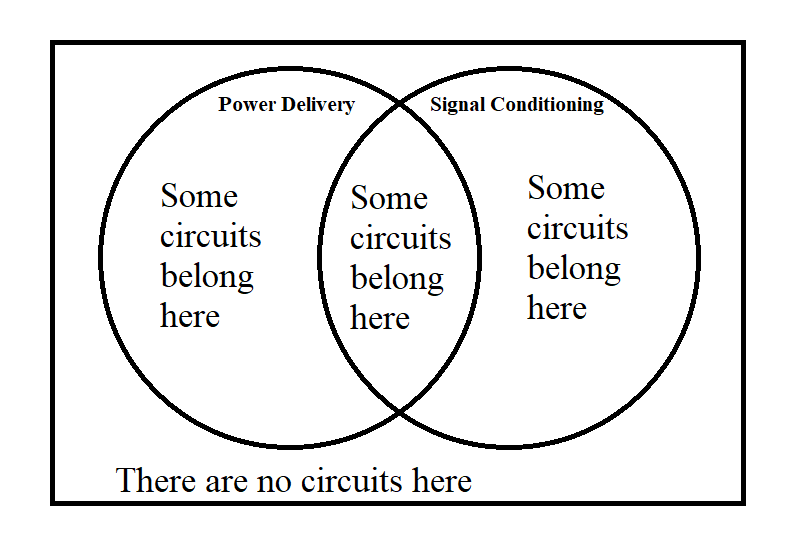
\includegraphics[width=15cm]{figures/vennDiag.png}
\caption{This comprehensive Venn diagram includes all the categories of circuits.}
\label{categoriesVennDiagram}
\end{figure}
\par
Because the categories of circuits are so few, linking the concepts in this course together should not be difficult. When you wonder why we are studying a specific topic, just think about the circuit categories; you will likely be able to connect the material in question to either powering devices or to conditioning signals. Furthermore, the first half of the class is almost exclusively about power delivery and dissipation. I hope these categories help you as we progress.
\par
After teaching introductory circuits for several years, I decided that most circuits textbooks aren't really written for you, the student; they're not fun to read\footnote{Yes, I know this is a course on circuits, but I still hope you'll enjoy reading these notes anyway.}, and they are really expensive. I wanted to write my own notes in lieu of assigning a textbook because I think everything in these notes is important (I wrote it all, so I wouldn't have gone to the trouble if I didn't think it was worth it), I actually want you to read them, and I don't want you to have to sell enough plasma to buy a traditional textbook for this course. During our time together this semester, in addition to learning about circuits, you will be helping me make these notes better! Your assignments will include \textit{active reading}. By that I mean you will read sections of these notes, taking your own notes while you go. In your notes, I especially want you to write questions that you wish the text would answer. This will give me valuable information when I revise my notes, and it will also help you interact with the material before we meet together. Yay! Thank you in advance for your help, and I hope you enjoy the course!